\documentclass[WHATMANUAL.tex]{subfiles}

\begin{document}

\chapter{Introduction}

\section{What is WHAT}

WHAT (Well Hydrograph Analysis Toolbox) is a free, open source, and cross-platform interactive computer program whose main focus is the interpretation of observation well hydrographs, including:

\begin{itemize}

\item the preparation of a gapless daily weather time-series (precipitation and air temperature) representative of the well location. For this purpose, an interface to the online Canadian Daily Climate Database (CDCD) is provided that allows to query stations interactively by location coordinates, download the available data, and automatically rearranged the data in a format compatible with WHAT. Furthermore, missing data for a given station can be quickly filled with data from selected neighboring weather stations using a multiple linear regression model;

\item the generation of various publication-quality figures from the weather and water level data;

\item the exploration, manipulation, and validation of the data within a user-friendly dynamic graphical environment;

\item the calculation of the master recession curve of the well hydrograph (experimental);

\item the estimation of groundwater recharge at the local scale in unconfined conditions with a method combining the daily meteorological data and the water level time series (will be available in a future release).

\item the calculation of the barometric response function of the well that can be used to assess the level of confinement of the aquifer at the well location (will be available in a future release).

\end{itemize}

WHAT is written in the Python 2.7 programming language and is currently maintained and developed by Jean-S\'ebastien Gosselin at INRS-ETE (\url{www.ete.inrs.ca}). The source code and a stand-alone executable for Windows 7 are available free of charge for download on GitHub (\url{https://github.com/jnsebgosselin/WHAT}). If you encounter any problems or errors during program execution, have any questions, or have specific suggestions on how to improve WHAT, please contact Jean-S\'ebastien Gosselin at this email address \href{mailto:jnsebgosselin@gmail.com}{jnsebgosselin@gmail.com}.

\newpage

\section{Installation}\label{sec:intallation}

WHAT can run on Windows, Linux, or OS X computer operating systems. However, a stand-alone executable of the program is currently released and tested only for the Windows 7 platform. This executable should also be compatible with Windows XP. For the Linux and OS X platforms, the software can be run directly from the source code, provided that Python 2.7 and all the required third party packages are installed on the computer (PySide, NumPy, matplotlib, xlrd, xlwt).

The stand-alone executable for Windows 7 is distributed in a Zip archive that can be downloaded freely on GitHub (\url{https://github.com/jnsebgosselin/WHAT/releases}). This archive contains:

\begin{itemize}

\item the GNU General Public License;

\item a folder named ``WHAT'' that contains all the necessary system files for the program to run, including the file ``WHAT.exe'' from which the software can be started;

\item a folder named ``Projects'' where all input and output files used or created by WHAT are stored by default. In this folder are included samples of input and output files that provide a quick and convenient way to test and learn the various features of the program.

\end{itemize}

Once the content of the Zip archive has been extracted, the program can be started directly from the WHAT.exe executable file that is contained withing the folder named WHAT. The software can conveniently run from any location on the computer or from any storage device without the need to install the program beforehand.

\section{Overview of the Graphical User Interface}
\label{sec:GUI_overview}

%There is no traditional menus in WHAT and everything is instead displayed within a menu bar that is located at the top of the interface.

WHAT Graphical User Interface (GUI) mainly consists of a menu bar, a console area, and a central view panel (see Figure~\ref{fig:WHAT_GUI}). The \emph{menu bar} is located in the top right corner of WHAT main window. This is where you can view what is the current project, open an already existing project or create a new one. The \emph{console} is located at the bottom of the WHAT interface and is used to report technical information about the various tasks accomplished by the program as well as warning and error messages. The console can be collapsed to save space, or can be extended to the entire window area. The \emph{central view panel} is the main component of the WHAT interface and is where are displayed the various features of the software. The content of this panel is divided into four tabs: \emph{Download Data}, \emph{Fill Data}, \emph{Hydrograph}, and \emph{About}. The tabs are described in a little bit more details in the text below and are shown in Figure~\ref{fig:WHAT_GUI_ScnShot}.

\begin{figure}[!ht]
\centering
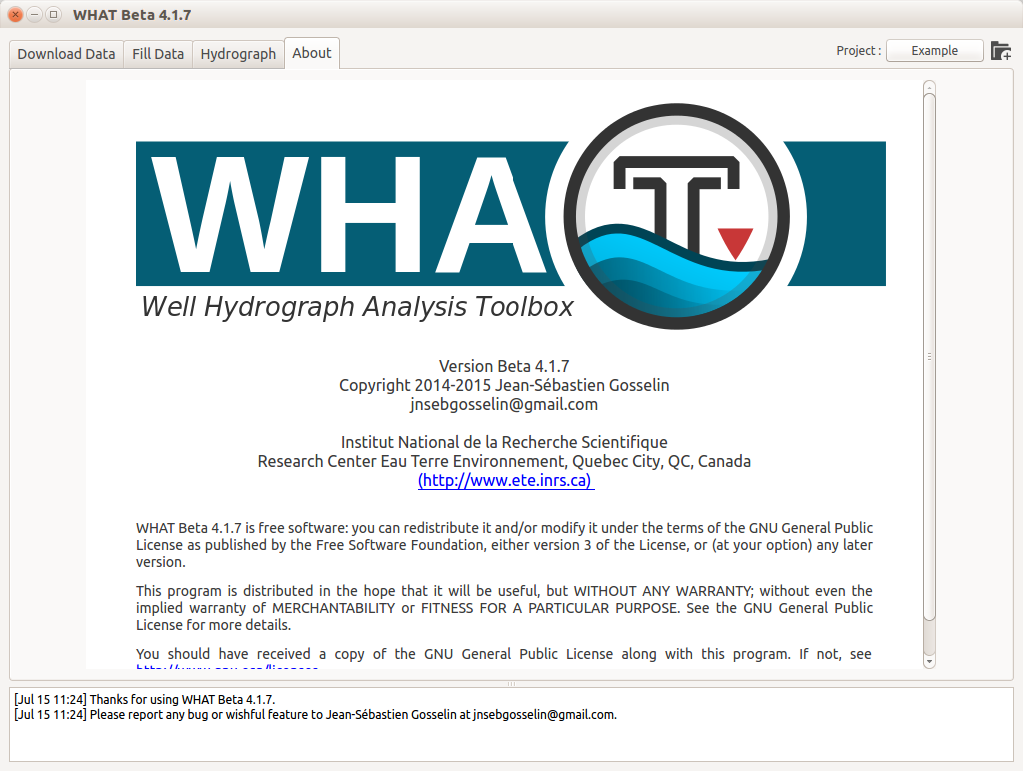
\includegraphics[width=0.75\textwidth]{img/WHAT_GUI}
\caption[WHAT GUI main features.]{WHAT GUI main features.}
\label{fig:WHAT_GUI}
\end{figure}

\newpage

\paragraph{Download Data} This tab (see Figure~\ref{subfig:ScnShot_000}) provides an interface to the online Canadian Daily Climate Database (CDCD) that allows to query stations interactively by location coordinates, download the available data, and automatically rearranged the data in a format compatible with WHAT. Alternately, it is possible to provide a custom list of Canadian weather stations for which data can be downloaded and formatted. At the moment, it is not possible to access data of weather stations located in the U.S. This feature may be added in a future release of the software.

\begin{figure}[!ht]
        \centering
        \begin{subfigure}[t]{0.45\textwidth}
                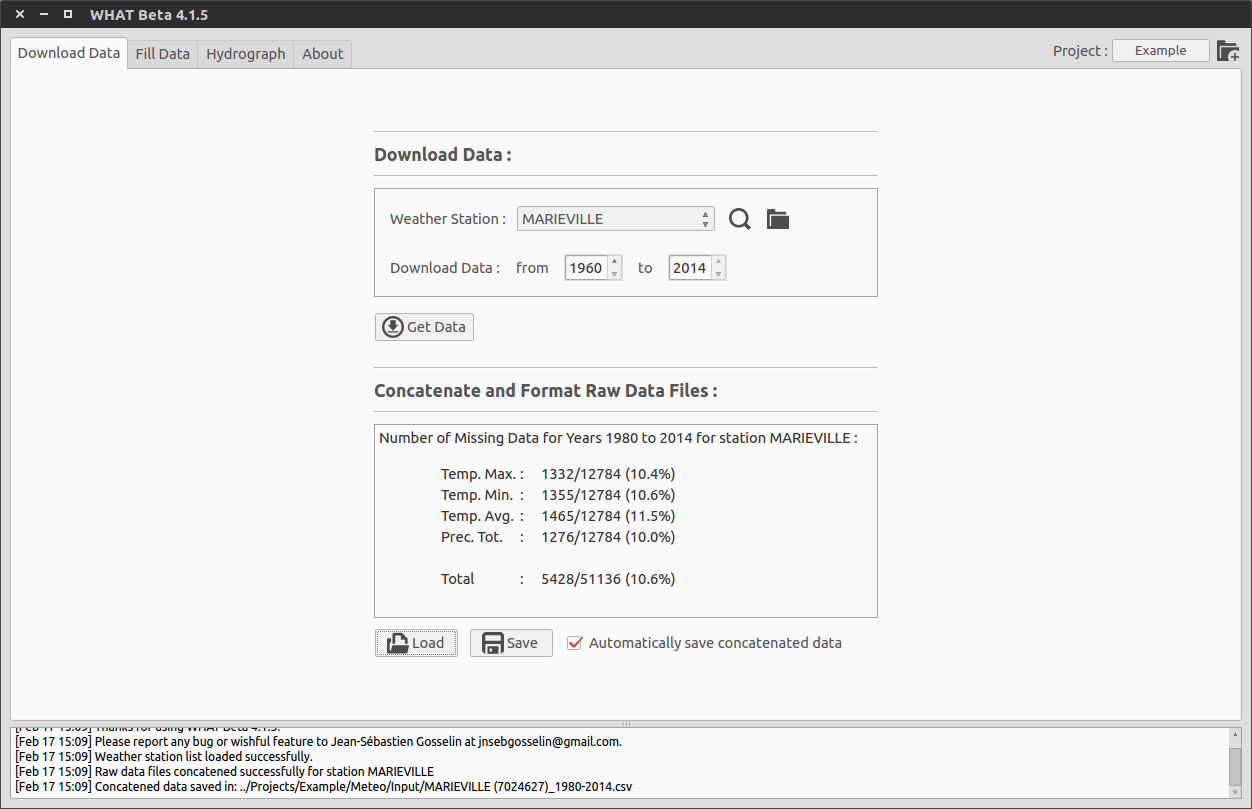
\includegraphics[width=\textwidth]{img/WHAT_Screenshot000}
                \caption{``Download Data'' tab.}
                \label{subfig:ScnShot_000}                
        \end{subfigure}%
        \hspace{0.5cm}
        \begin{subfigure}[t]{0.45\textwidth}
                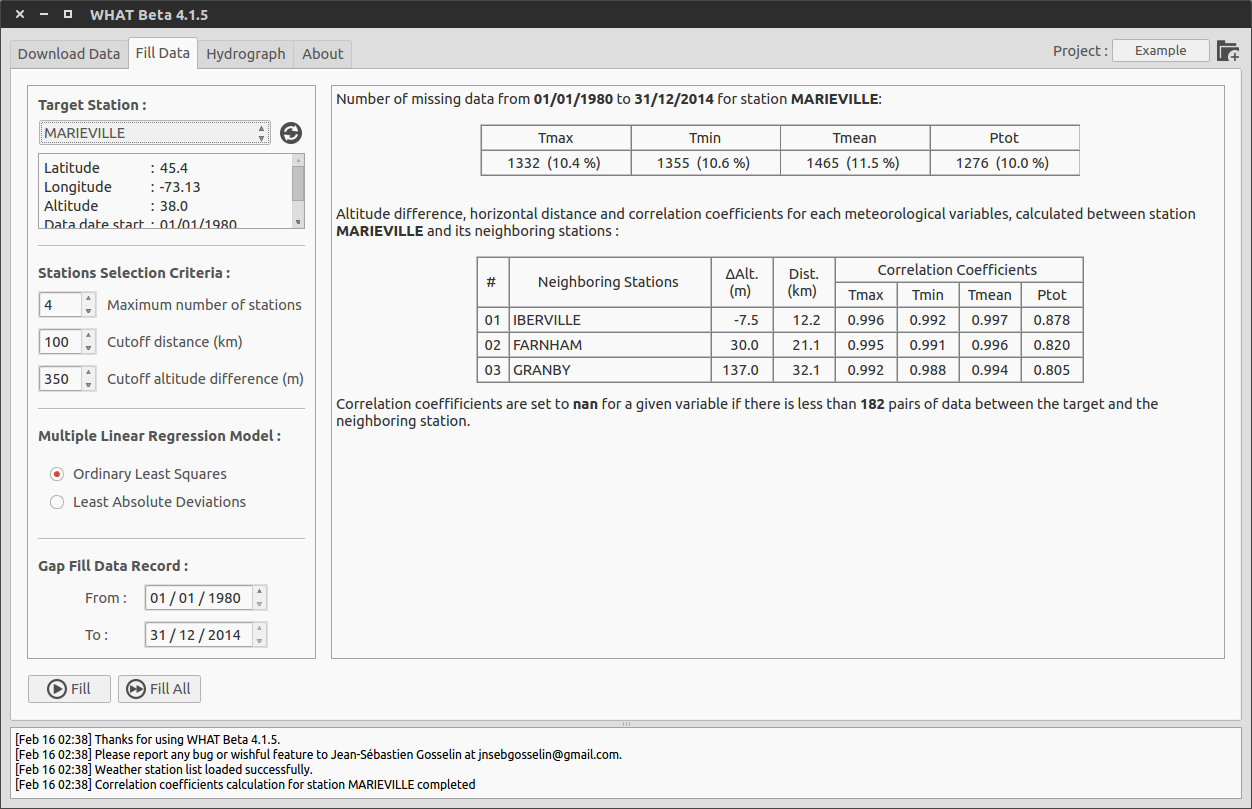
\includegraphics[width=\textwidth]{img/WHAT_Screenshot001}
                \caption{``Fill'' Data tab.}
                \label{subfig:ScnShot_001}
        \end{subfigure}
        \\[0.5cm]
        \begin{subfigure}[t]{0.45\textwidth}
                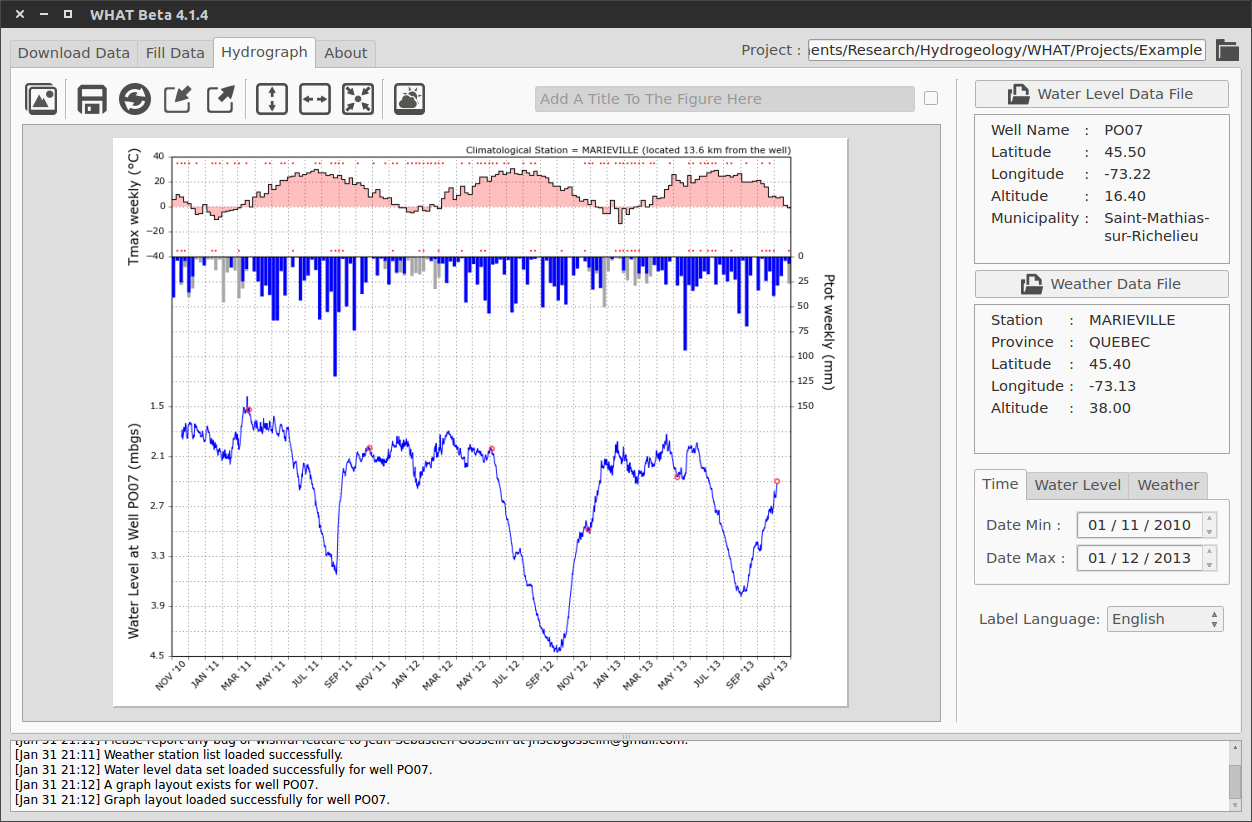
\includegraphics[width=\textwidth]{img/WHAT_Screenshot002}
                \caption{``Hydrograph'' tab in mode ``Layout''.}
                \label{subfig:ScnShot_002}
        \end{subfigure}
        \hspace{0.5cm}
        \begin{subfigure}[t]{0.45\textwidth}
                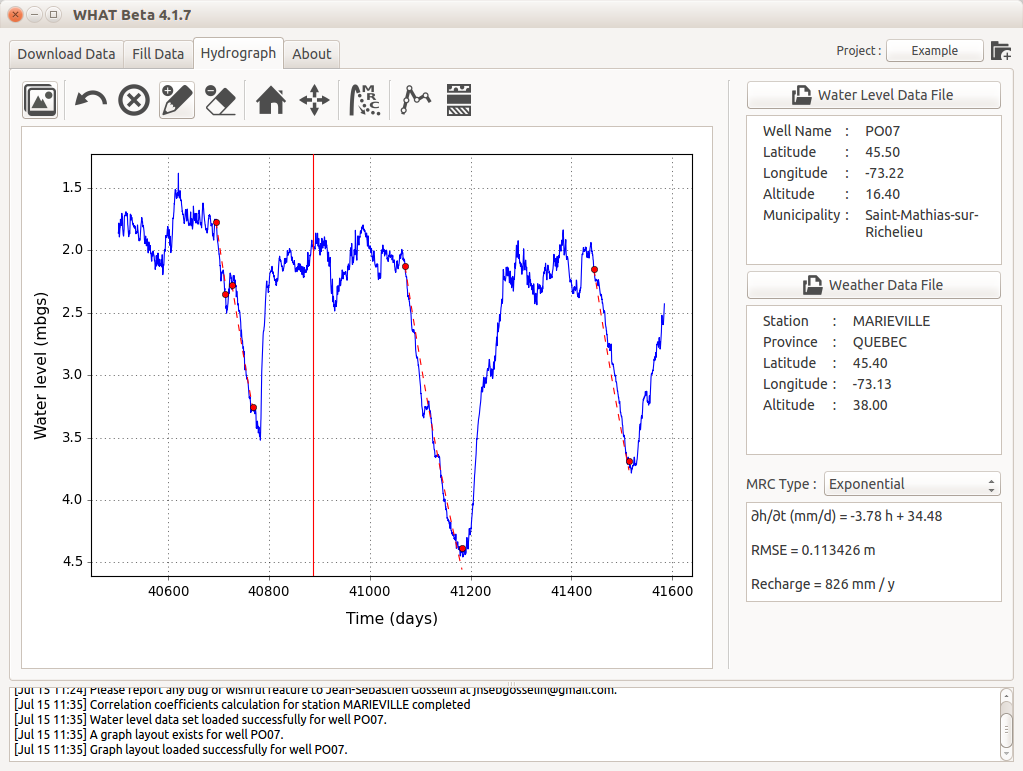
\includegraphics[width=\textwidth]{img/WHAT_Screenshot003}
                \caption{``Hydrograph'' tab in mode ``Computation''.}
                \label{subfig:ScnShot_003}
        \end{subfigure}
        \caption[Screenshots of WHAT GUI tabs captured in Ubuntu Linux 14.04.]{Screenshot of WHAT GUI tabs captured in Ubuntu Linux 14.04. (a) ``Download Data'' tab. (b) ``Fill'' Data tab (c) ``Hydrograph'' tab in mode ``Layout''. (d) ``Hydrograph'' tab in mode ``Computation''.}\label{fig:WHAT_GUI_ScnShot}
\end{figure}

\paragraph{Fill} This tab (see Figure~\ref{subfig:ScnShot_001}) is where you can automatically estimate the missing daily weather values in your data to create gapless time-series of daily precipitation and air temperature. Missing data for a given station are estimated from selected neighboring weather stations using a multiple linear regression model.

\paragraph{Hydrograph} This tab is used for viewing and plotting data. For this purpose, two modes are available: the \emph{layout} and the \emph{computation} mode. Both modes share the same weather and water level dataset and it is possible to switch from one mode to the other at anytime. The \textbf{layout} mode (see Figure~\ref{subfig:ScnShot_002}) provides an interface to interactively produce publication-quality graphs from the data. The \textbf{computation} mode (see Figure~\ref{subfig:ScnShot_003}) consists in a dynamic graphical environment where data can be explored, manipulated and analyzed. Various computational tools are available in this mode, including the estimation of the hydrograph Master Recession Curve (MRC) and the estimation of groundwater recharge.

\paragraph{About} This tab (see Figure~\ref{fig:WHAT_GUI}) displays copyright, licensing and general information about WHAT.

\section{Workflow for Interpreting Water-level Time-series}
\label{sec:workflow}

WHAT essentially consists of set of tools to assist the interpretation of water level time series measured in observation wells, from the preparation of raw data to the assessment of groundwater recharge when in unconfined conditions. In this perspective, WHAT was developed with the general workflow shown in Figure 6  in mind.

\begin{figure}[!ht]
\centering
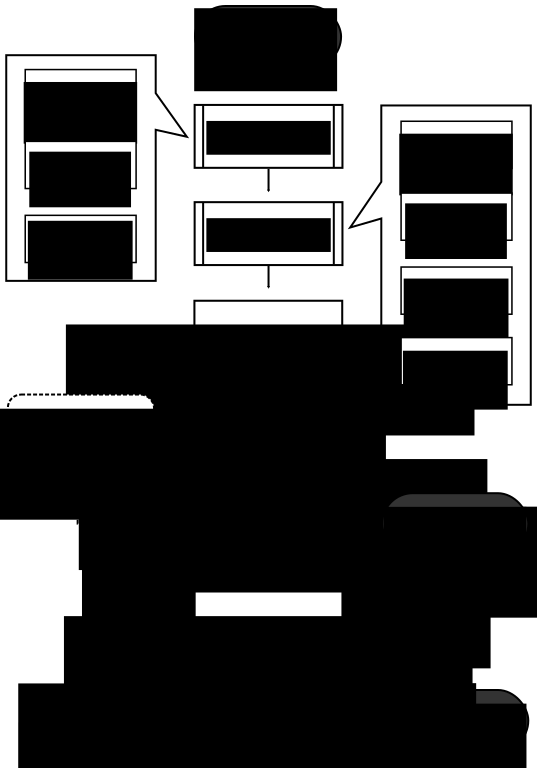
\includegraphics[width=0.95\textwidth]{img/WHAT_Workflow}
\caption[WHAT conceptual workflow.]{WHAT conceptual workflow for the interpretation of water-level time-series measured in an observation well.}
\label{fig:WHAT_workflow}
\end{figure}

The first step consists in the preparation of a gapless weather dataset.

Validation/preparation of water level time series: 1) automatic measurements fitted to manual measurements. 2) Correct the places where there is a break in the water level curve. This is due generally to the logger that is placed at a different level following the removal of the later from the well. 3) Remove measurements that were acquired while the barologger was outside the water column.

Preparation of a gapless weather dataset. This include. Downloading data from the CDCD database for stations located in a radius of 0 to 100 km from the well. Fill missing daily data for the station located closest to the well by using selected neighboring stations. Data are not interpolated to the exact location of the well. It has been decided to keep the original dataset of the station located closest to the well to analyse the data. This is due to the fact that conventional technique for interpoloating weather data tend to surestimate the number of wet day, but underestimate the intensity of stron precipitation event. More advanced and complicated technique are required to circumvent these issues. It has thus been decided that is was prefereable to keep the original data from a single station.

Once the weather data, and water level are prepared, production of a well hydrograph. Visual interpretation between the water level  fluctuation and weather data can be done.

If high time resolution measurement of the water level and barometric pressure are available, it is possible to carry an calculation of the barometric response function. It is also good to produce a FFT analysis of the hydrograph.
Weather yearly average and montlhy averages can be plotted at this stage.
If the visual inspection of the well, and the barometric response function, determined that the well in unconfined, it means groundwater recharge can be estimated from the data. First, determining the segment where groundwater recharge can be supposed to be negligible and where the water level recede. After that, compute the MRC, and compute a first estimation of groundwater recharge using the Water-Table Fluctuation principle. Estimate finaly recharge with a method combining the meteorological data and the well hydrograph. Enjoy.

\end{document}